\documentclass{beamer}

\setbeamertemplate{navigation symbols}{}

\usepackage{graphicx}
\usepackage{amsmath, amssymb, amsfonts, amsthm}
\usepackage{tabularx}

\usetheme{CambridgeUS}


%-----------------------------------------------------------------------------------------------------------------
% New Environment for a plain box
\newenvironment{boxeded}
    {\begin{center}
    \begin{tabular}{|p{0.9\textwidth}|}
    \hline\\
    }
    { 
    \\\\\hline
    \end{tabular} 
    \end{center}
    }
%-----------------------------------------------------------------------------------------------------------------

% Die Präsentation dient dem Praxisprojekt: COVID-19 und wurde von Regina Galambos und Lorenz Mihatsch erstellt.

% Folgende Inhalte sollen besprochen werden: 
% 1: Datenstruktur und -erhebung erläutern:
% 1.1) Probleme der Erhebung: Recoding policy, testing policy.
% 2: Fallzahlen Weltweit als Timescale und als Weltkarte bezogen auf 100k Einwohner
% 3: Wachstumsraten der Fallzahlen
% 4: Ländervergleich. Zentrieren um Tag der Abriegelung irgendeiner Art.






%-----------------------------------------------------------------------------------------------------------------
% Presentation information: title, author.....

\title[Praxisprojekt: COVID-19]{Analyse der COVID-19 Fallzahlen}
\subtitle{Praxisprojekt}
\author[R.Galambos, L.Mihatsch]{Regina Galambos, Lorenz Mihatsch\\
	
\includegraphics[width=0.22\textwidth]{LMU.pdf}\\
	{\small Projektpartner: Andr\'{e} Klima}}
%-----------------------------------------------------------------------------------------------------------------


%-----------------------------------------------------------------------------------------------------------------
% Begin of presentation.

%Title page
\begin{document}
\begin{frame}
	\titlepage
\end{frame}

% Table of contents
\begin{frame}
   \frametitle{Inhaltsangabe}
   \tableofcontents
 \end{frame}
 
 
 % Einführung
 %-----------------------------------------------------------------------------------------------------------------
 \section{Einführung}
 \begin{frame}
 	\frametitle{COVID-19 Pandemie}
 	\begin{enumerate}
 		\item COVID-19 ist ein Erkrankung die durch das SARS-CoV-2 Virus ausgelöst wird.
 		\item Die Erkranung ist erstmalig im Dezember 2019 in Wuhan (China) aufgetreten, der genaue Ursprung ist jedoch noch immer unbekannt.
 		\item Erster Fall in Deutschland am 28. Januar in Stockdorf.
 		\item Am 11.März wurde die ursprüngliche Epidemie als Pandemie eingestuft.
 		\item Am 22. März einigten sich Bund und Länder auf eine umfassende Beschränung sozialer Kontakte.
 	\end{enumerate}
 \end{frame}
 \section{Daten}
  
 \begin{frame}
 	\frametitle{Datesätze}
 	\begin{enumerate}
 		\item Falldaten einzelner Länder
 		\begin{itemize}
 			\item Datensatz des \emph{Centers of Systems Science and Engineering} der John Hopkins University. 
 			\item Täglich von \emph{RamiKrispin} auf GitHub aktualisiert und als long-Format zu Verfügung gestellt. \url{https://github.com/RamiKrispin/coronavirus}
 		\end{itemize}
 		\item Demographische Daten
 		\begin{itemize}
 			\item Datenbank der Weltbank. Zugriff über \emph{webstat}-Package.
 		\end{itemize}
 		\item Politische Maßnahmen
 		\begin{itemize}
 			\item Manuelle Recherche.
 		\end{itemize}
 	\end{enumerate}
 	\emph{Anmerkung}: Es handelt sich "nur" um die aufgezeichneten Fälle. Es wird von einer weitaus höheren Dunkelziffer ausgegangen.
 \end{frame}

 \begin{frame}
 	\frametitle{Anmerkungen}
 	\begin{enumerate}
 		\item Diamond Princess und MS Zaandam wurden ausgeschlossen.
 		\item Die Anzahl an Cases beziehen sich meist auf 100.000 Personen.
 		\item Programmierung einer Web-Application: url!!!
 	\end{enumerate}
 \end{frame}
 
 \section{Weltweit}
 \begin{frame}
 	\frametitle{COVID-19 weltweit}
	\begin{figure}
		\centering
		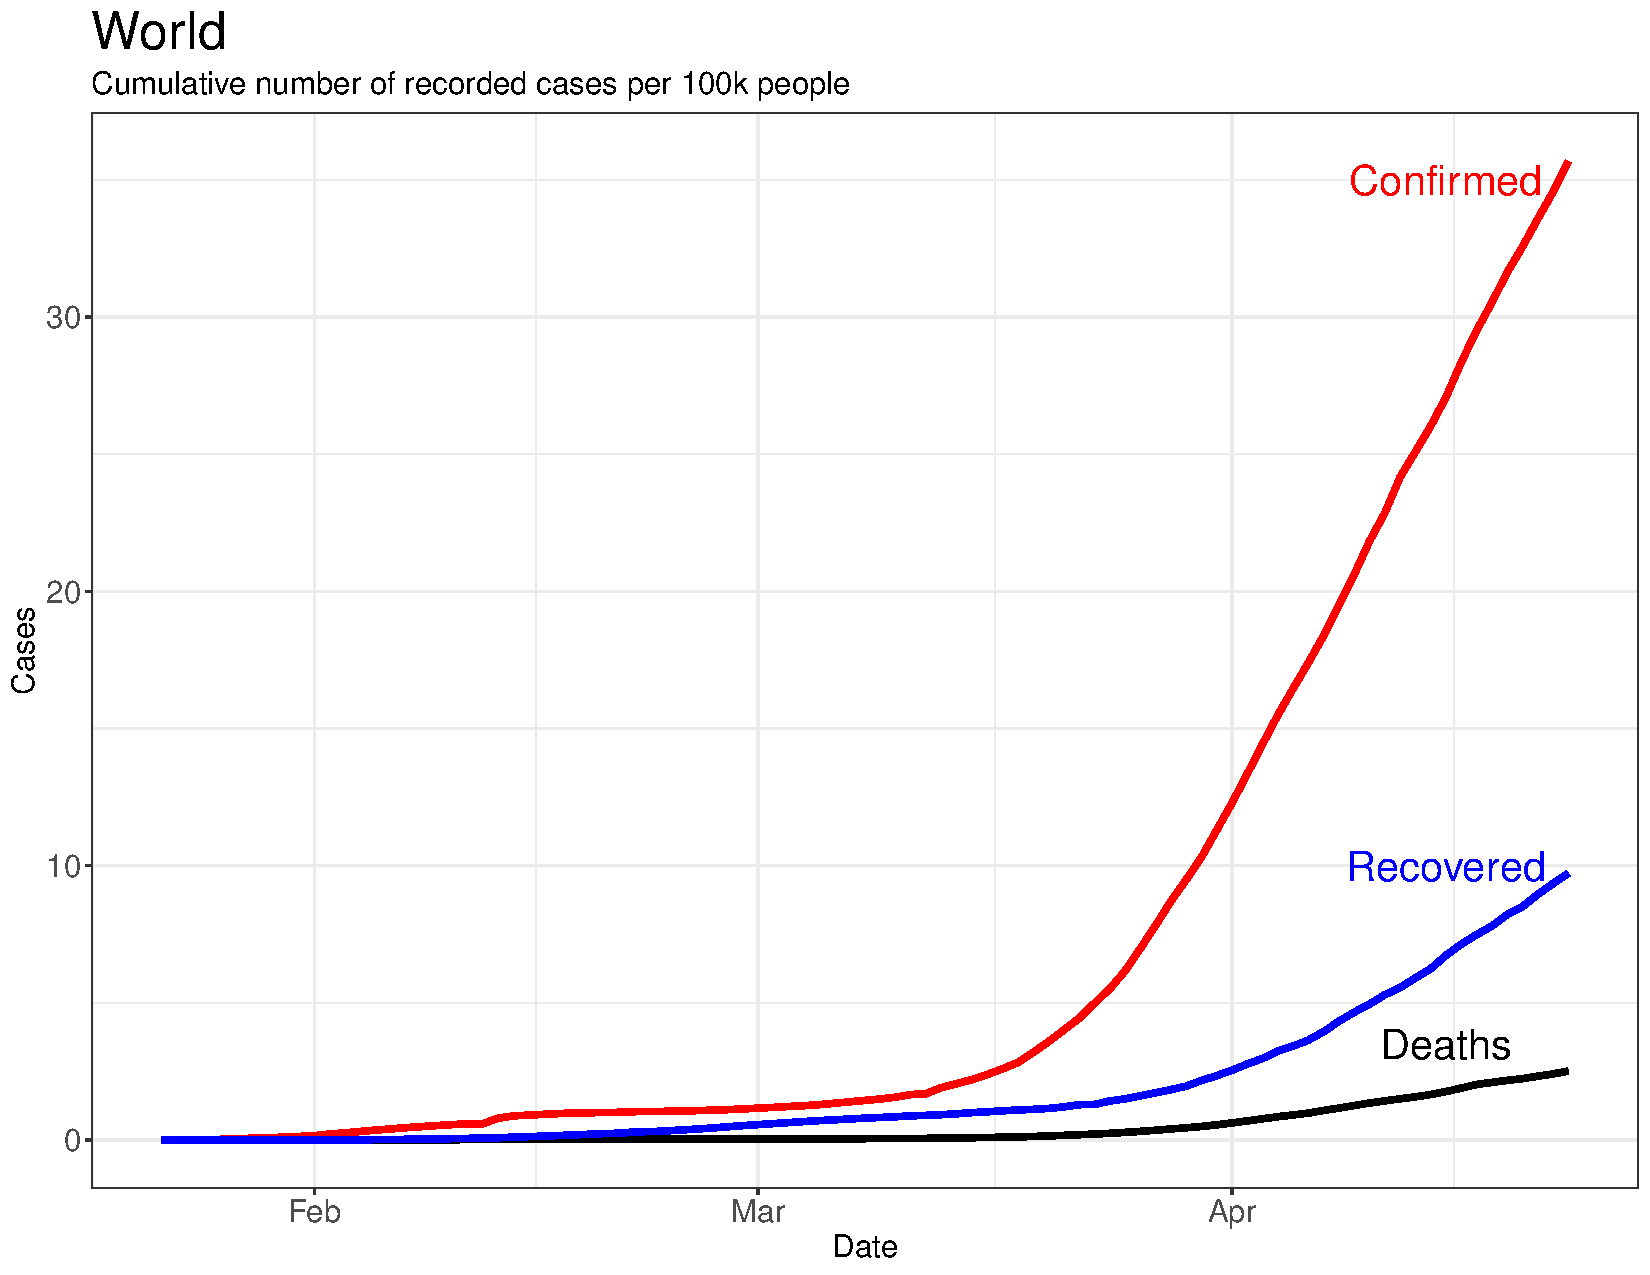
\includegraphics[width = 270pt]{Cases_world.pdf}
	\end{figure}
 \end{frame}

 \begin{frame}
 	\frametitle{COVID-19 weltweit}
	Kommentar: Hier die Weltkarten.
 \end{frame}
 
 \begin{frame}
 	\frametitle{COVID-19 weltweit bestätigte Fälle}
	\begin{figure}
		\centering
		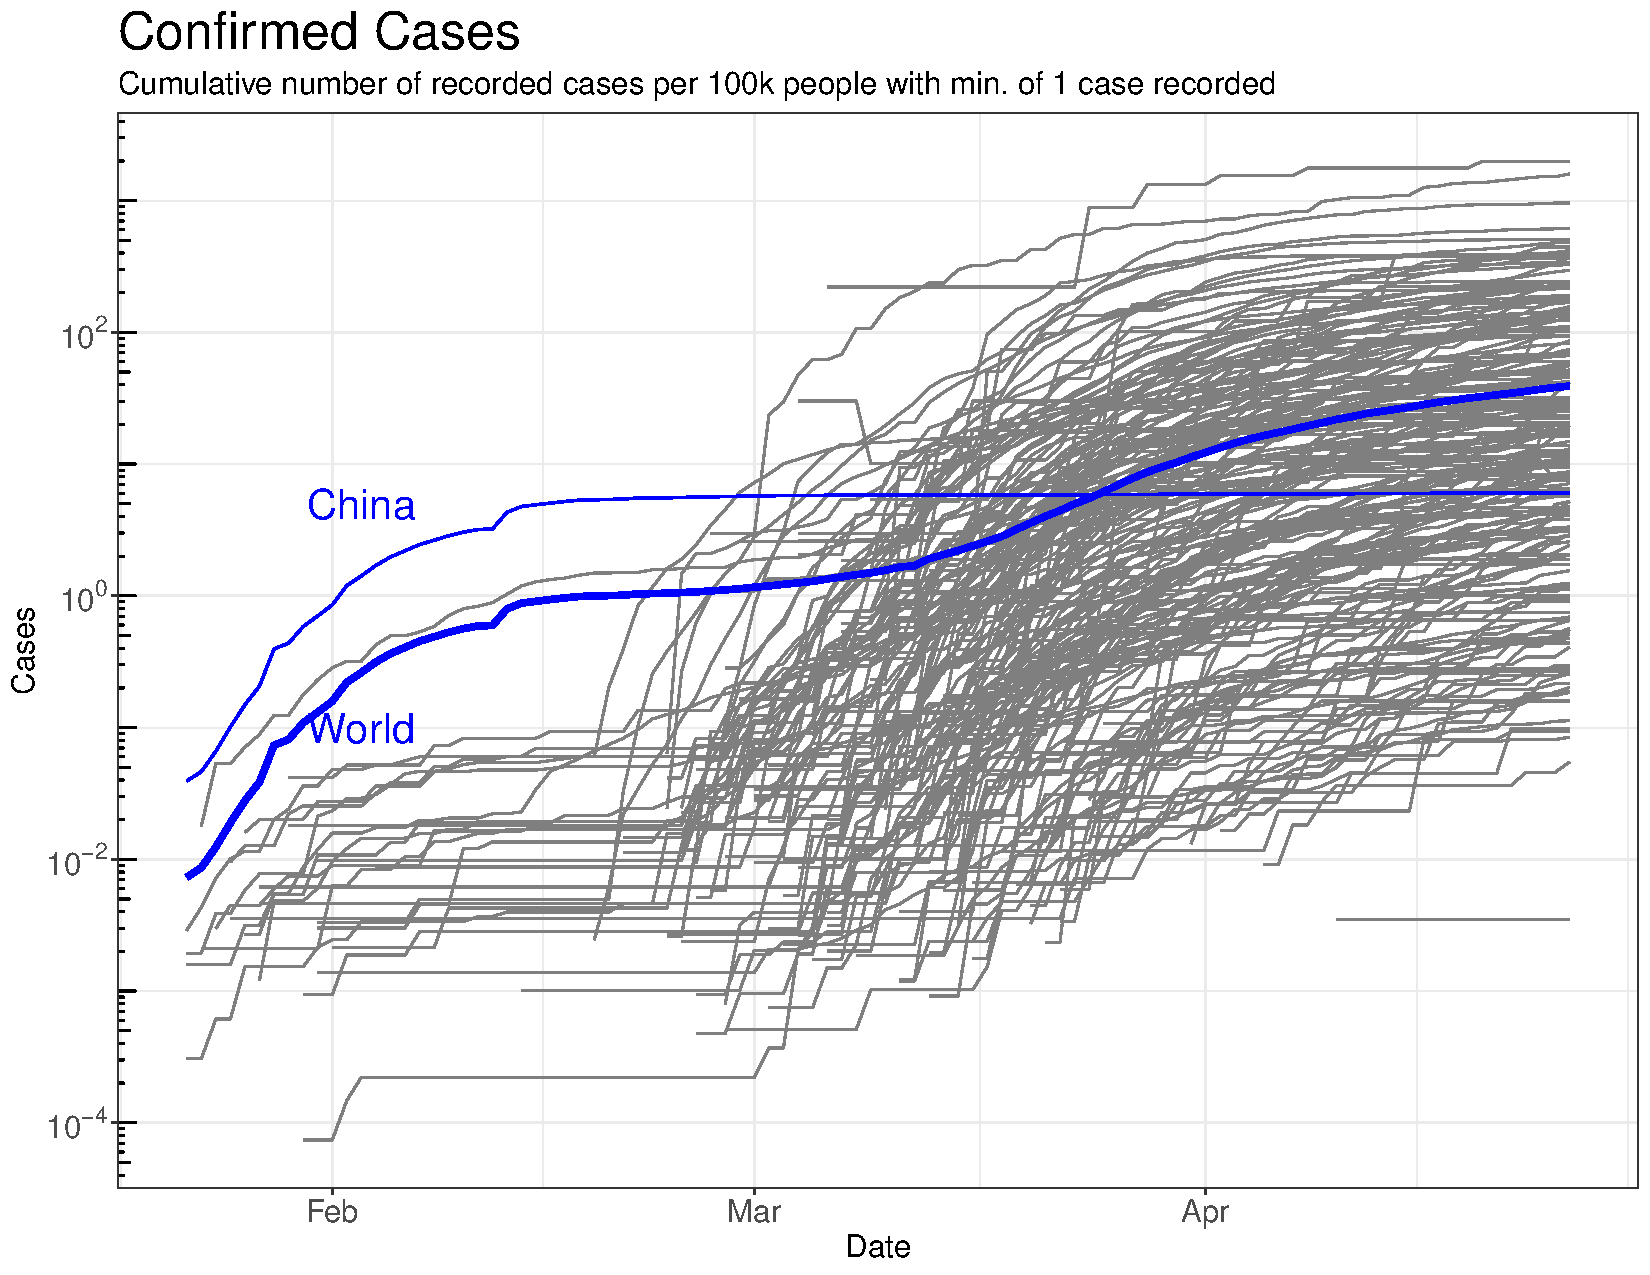
\includegraphics[width = 270pt]{Cases_cumulative_confirmed.pdf}
	\end{figure}
 \end{frame}

 \begin{frame}
 	\frametitle{COVID-19 weltweit bestätigte Todesfälle}
	\begin{figure}
		\centering
		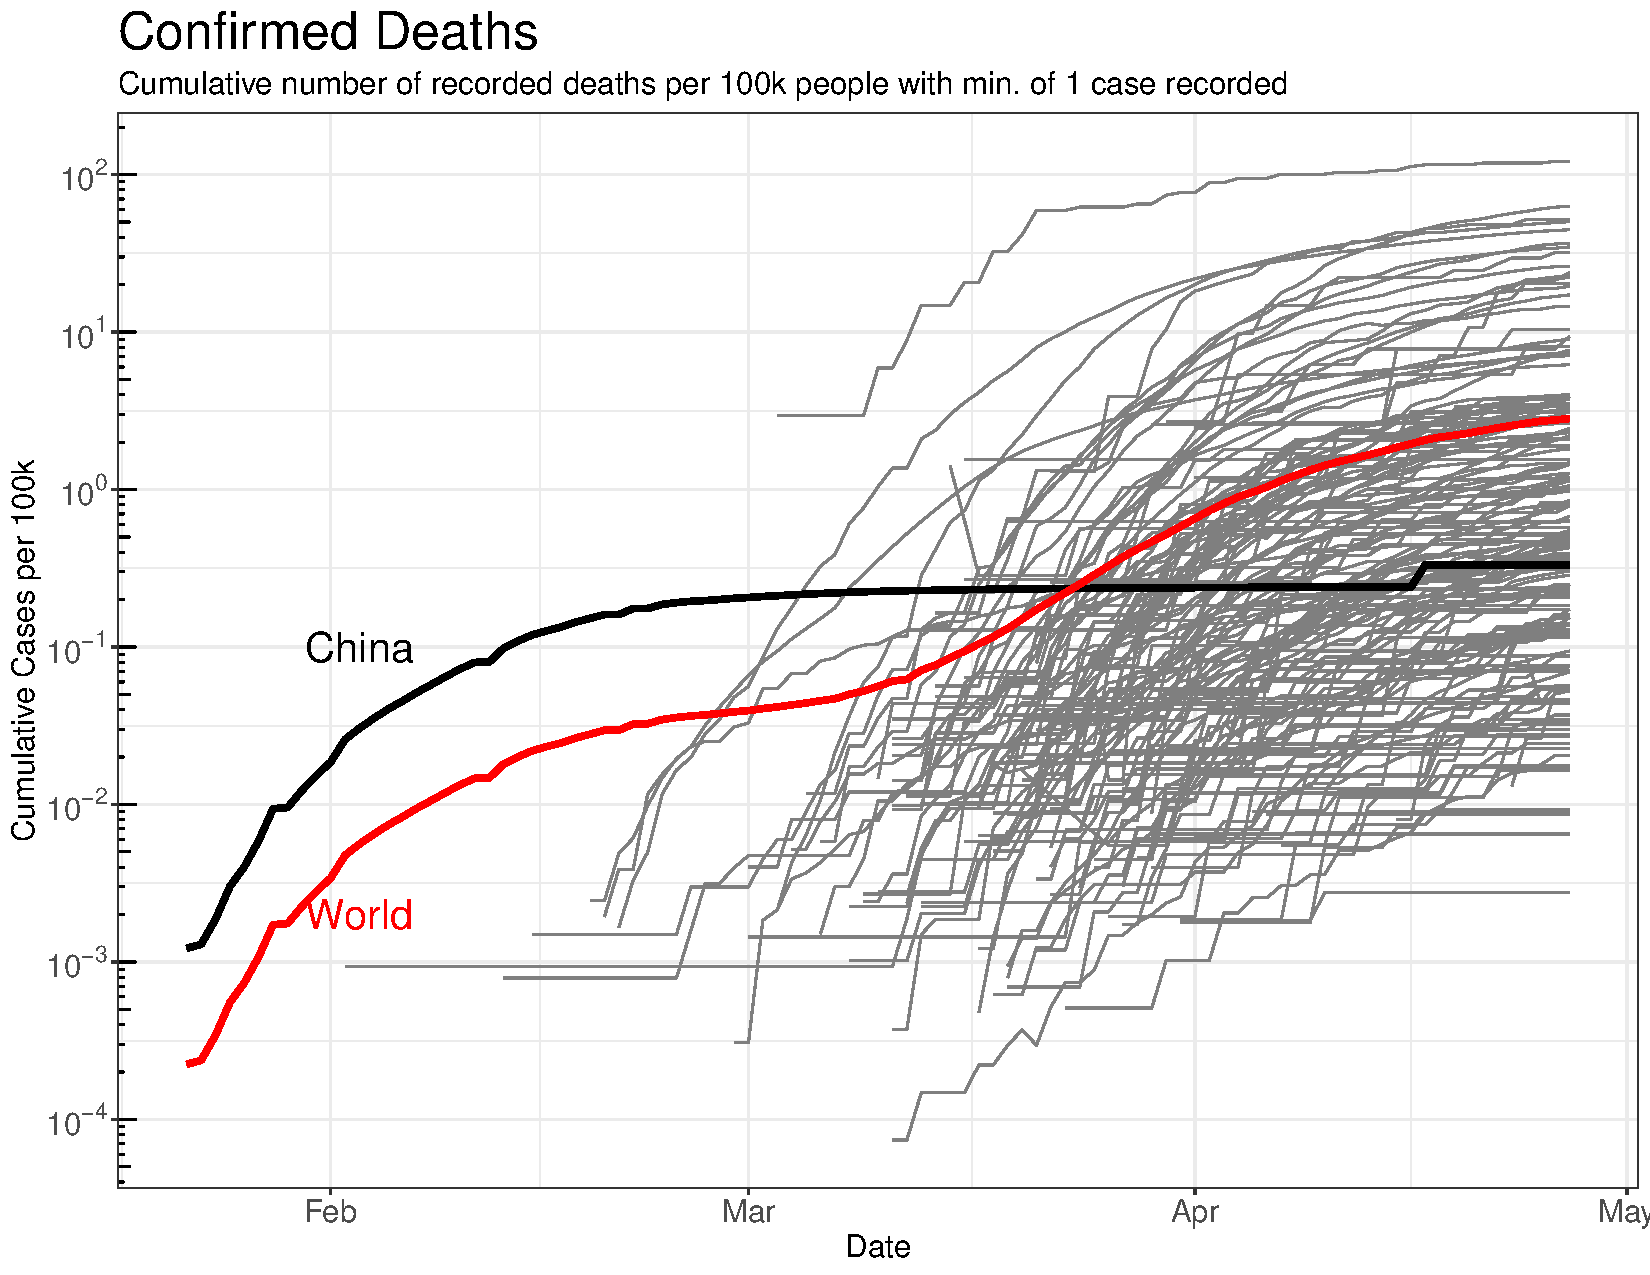
\includegraphics[width = 270pt]{Cases_cumulative_deaths.pdf}
	\end{figure}
 \end{frame}

 \begin{frame}
 	\frametitle{Zwischenergebnis}
 \end{frame}

\section{Wachstumsfaktoren}
\begin{frame}
	\frametitle{Wiederholung: Wachstumsfaktor und geometrisches Mittel}
	\begin{boxeded}
		\textbf{Definition 1} \textit{Wachstumsfaktor}\\
		Sei $C_0, C_1, C_2, ...$ eine Zeitreihe von Fallzahlen zu den Zeitpunkten $0, 1, ..., n$. Dann ist für $i = 1, ..., n$ der i-te Wachstumsfactor $x_1$ gegeben durch $$ x_i = \frac{C_i}{C_{i-1}}.$$
	\end{boxeded}

	Die Fallzahlen $C_n$ zum Zeitpunkt $n$ sind gegeben durch $$C_n = C_0 \cdot x_1 \cdot x_2 \cdot ... \cdot x_n$$
\end{frame}

\begin{frame}
	\frametitle{Wiederholung: Wachstumsfaktor und geometrisches Mittel}
	\begin{boxeded}
		\textbf{Definition 2} \textit{Geometrisches Mittel}\\
		Das geometrische Mittel zu den Wachstumsfaktoren $x_1, x_2, ..., x_n$ ist gegeben durch $$\bar{x}_{geom} = (x_1 \cdot x_2 \cdot ... \cdot x_n)^{1/n}.$$ Daraus ergibt sich $C_n = C_0 \cdot x_1 \cdot x_2 \cdot ... \cdot x_n = C_0 \cdot (\bar{x}_{geom})^n$.
	\end{boxeded}
	\pause
	Wir betrachten im Folgenden den \emph{rolling geometric mean} der vergangenen 7 Tage. Dazu berechnen wir für jeden Zeitpunkt $i$ $$\bar{x}_{i, geom} = (x_i \cdot x_{i-1} \cdot x_{i-2} \cdot ... \cdot x_{i-6})^{1/7}.$$
\end{frame}

\begin{frame}
	\frametitle{Wachstumsfaktoren: Bestätigte Fälle}
	\begin{figure}
		\centering
		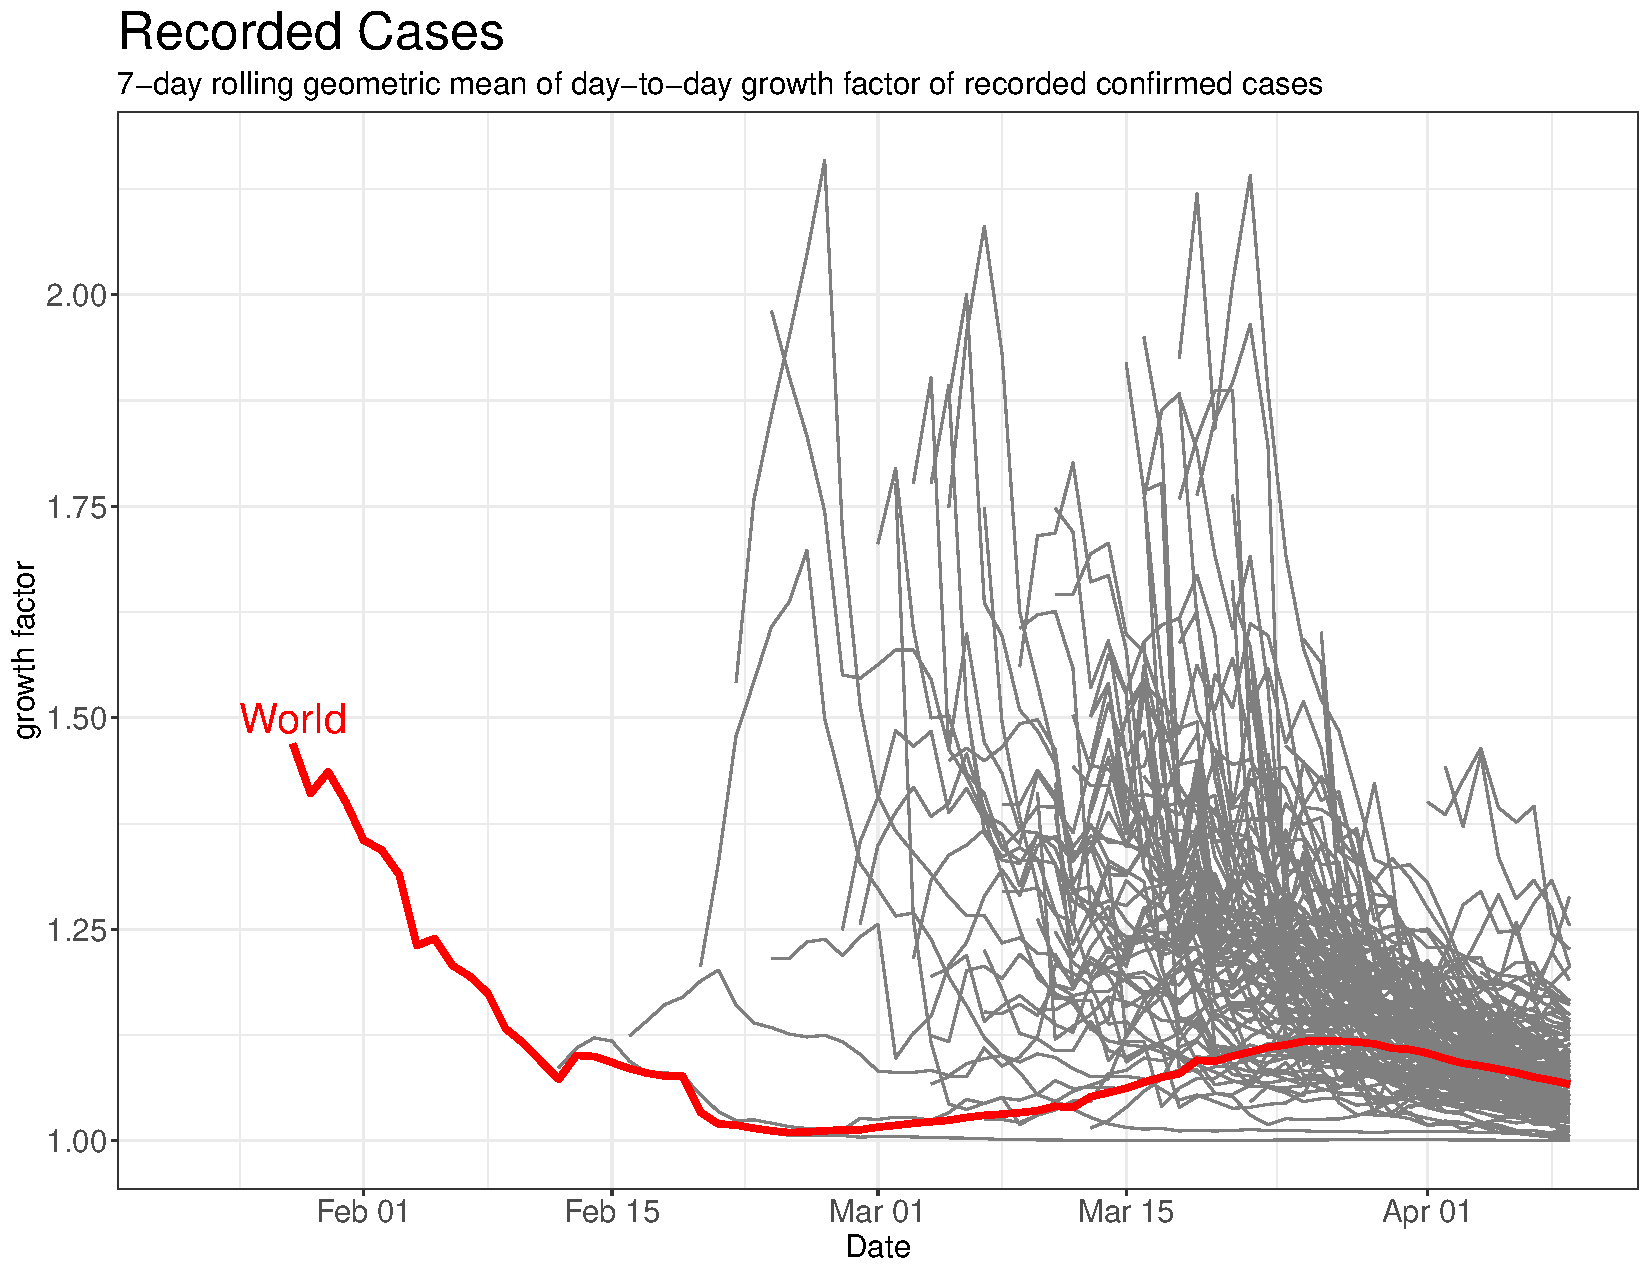
\includegraphics[width = 270pt]{GF_confirmed}
	\end{figure}
\end{frame}

\begin{frame}
	\frametitle{Wachstumsfaktoren: Todesfälle}
	\begin{figure}
		\centering
		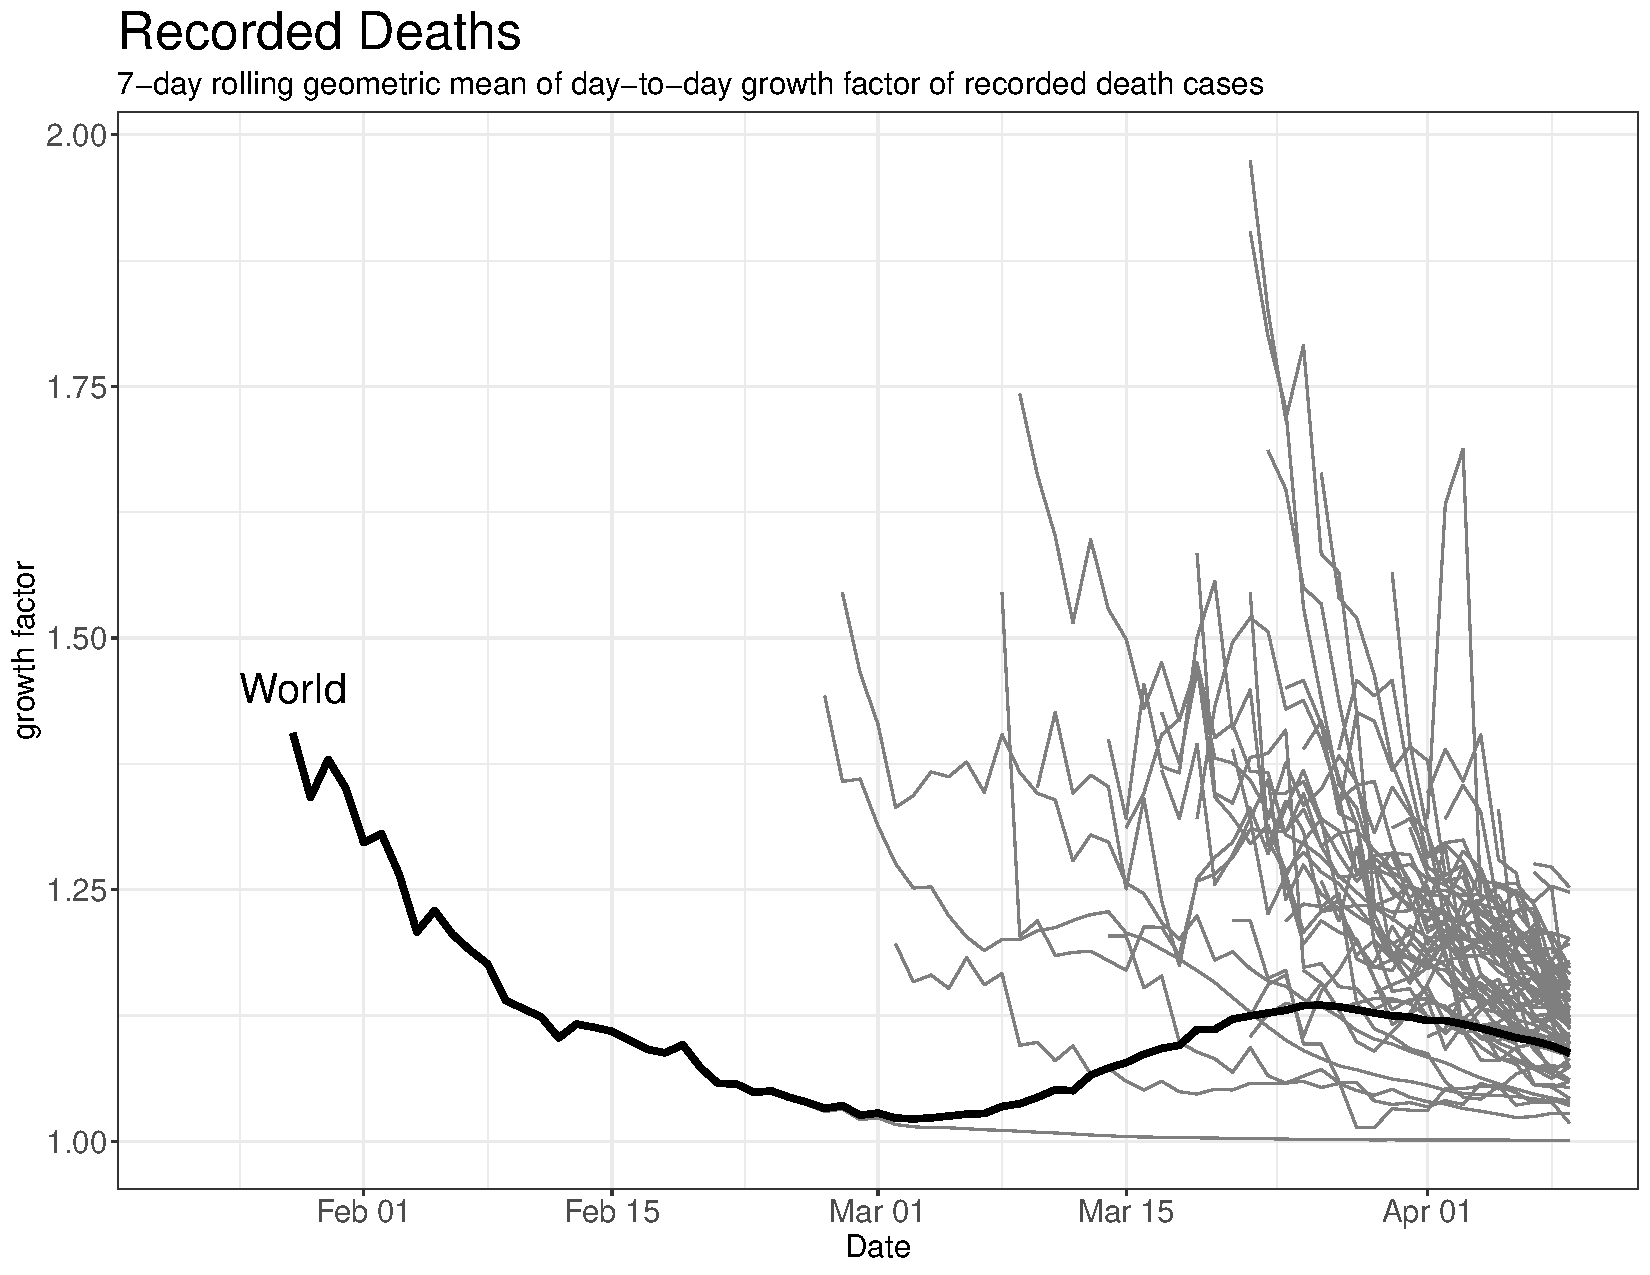
\includegraphics[width = 270pt]{GF_deaths}
	\end{figure}
\end{frame}

\begin{frame}
	\frametitle{Verdopplungszeit}
	Ausgehend von einem exponentielle Wachstum der Form $C_n = C_0 \cdot (\bar{x}_{n, geom})^{n}$ ergibt sie die "momentane" Verdopplunszeit $dt_i$ der Fallzahlen durch $$dt_i = \frac{ln(2)}{ln(\bar{x}_{i, geom})}.$$
	\pause
	\emph{Herleitung}: 
	\begin{align*} C_i \cdot (\bar{x}_{i, geom})^{dt_i} = 2 \cdot C_i 
		 &\iff (\bar{x}_{i, geom})^{dt_i} = 2 \\
	 	&\iff dt_i = \frac{ln(2)}{ln(\bar{x}_{i, geom})}.
	\end{align*}
\end{frame}

\begin{frame}
	\frametitle{Verdopplungszeit: Bestätigte Fälle}
	\begin{figure}
		\centering
		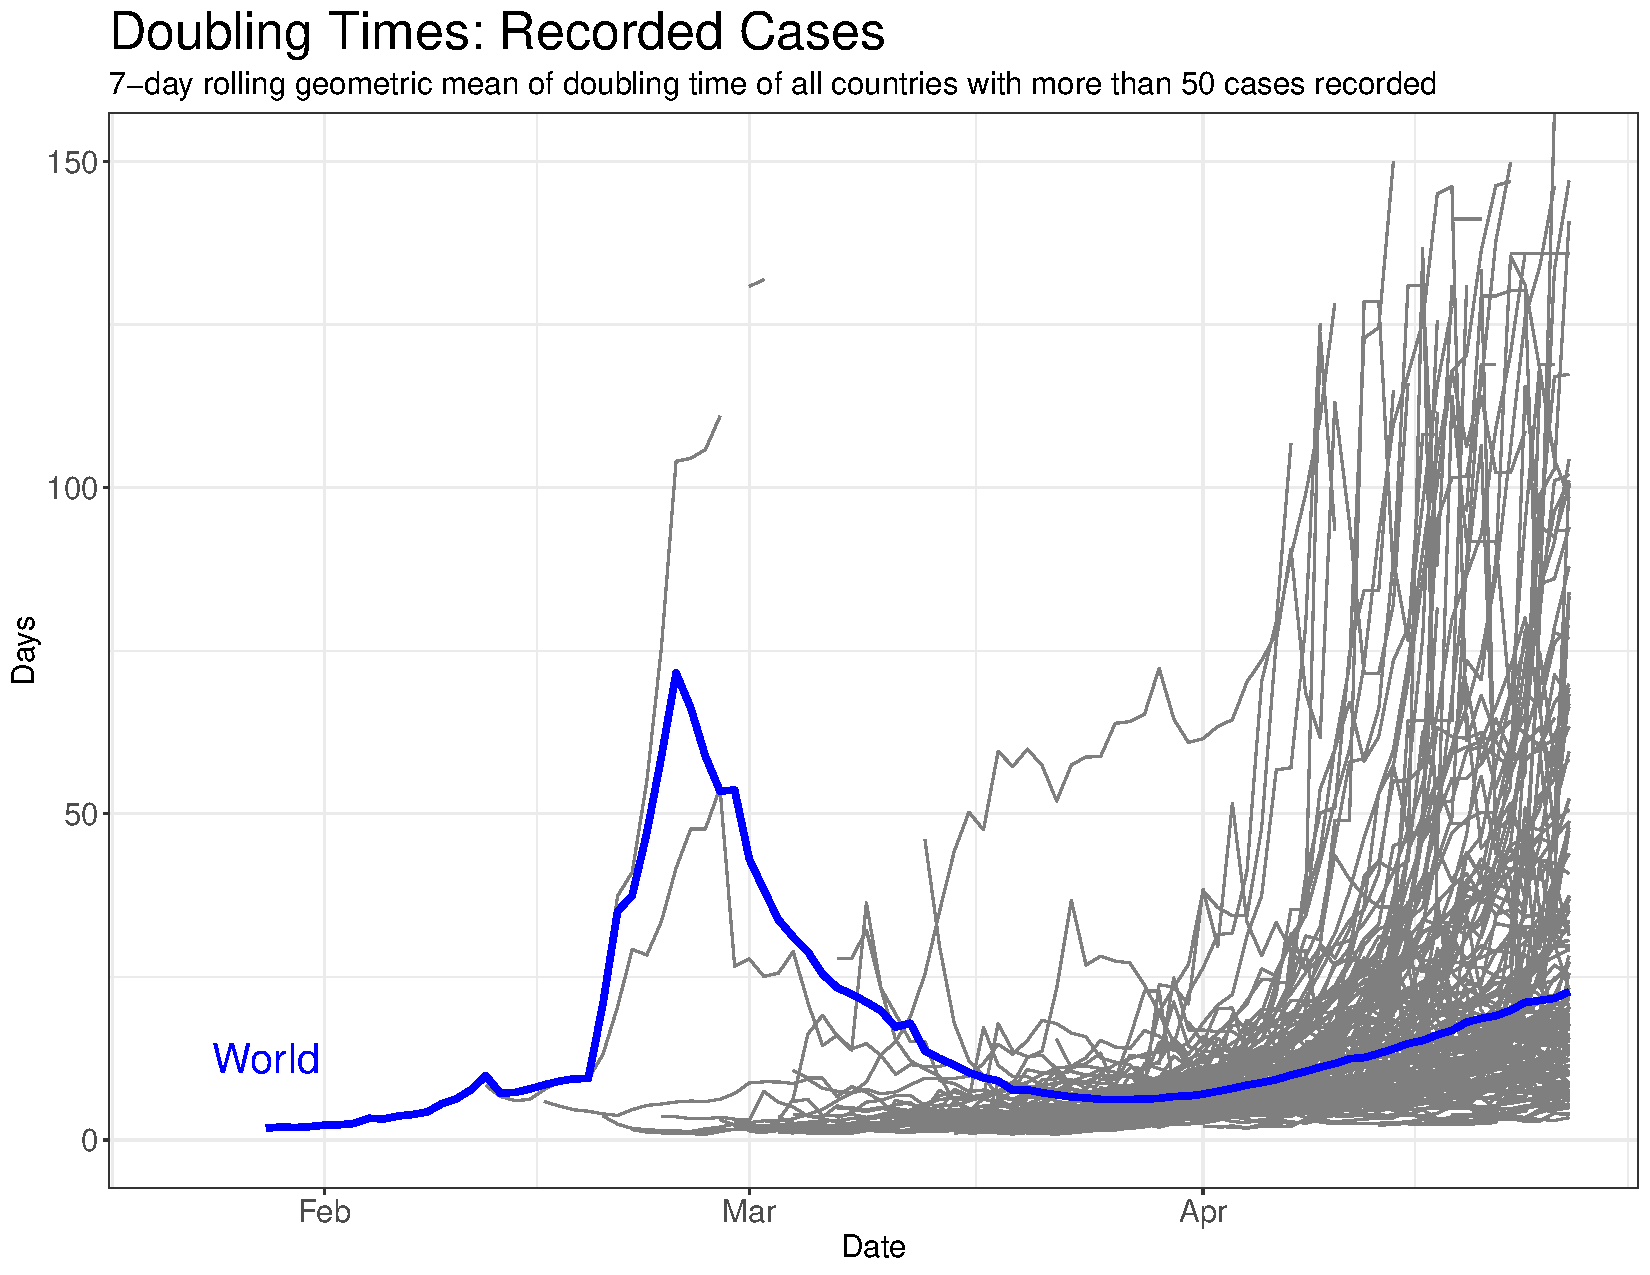
\includegraphics[width = 270pt]{DT_confirmed}
	\end{figure}
\end{frame}

\begin{frame}
	\frametitle{Verdopplungszeit: Todesfälle}
	\begin{figure}
		\centering
		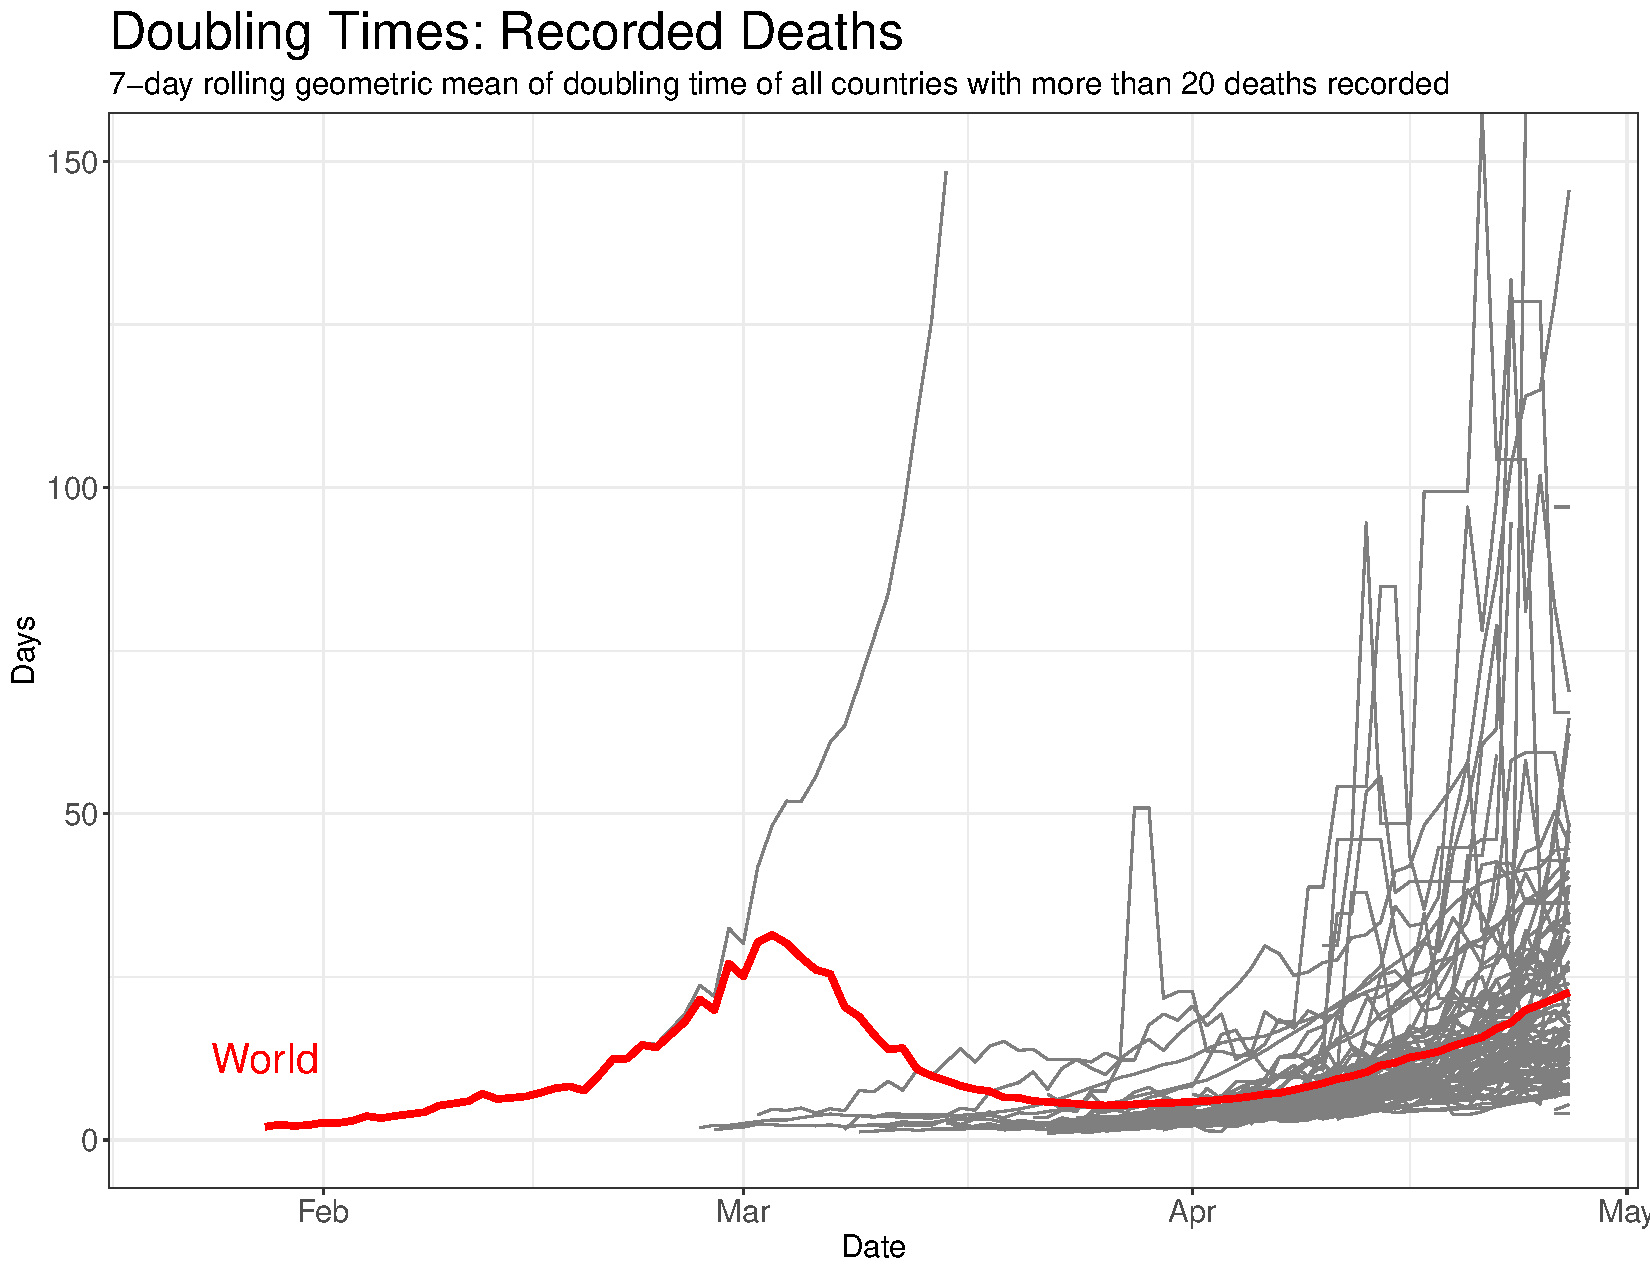
\includegraphics[width = 270pt]{DT_deaths}
	\end{figure}
\end{frame}

 \begin{frame}
 	\frametitle{Zwischenergebnis}
 \end{frame}

\section{Ländervergleich}
\begin{frame}
	\frametitle{Infektionsmaßnahmen}
	Kommentar: Beispiel Plot von South Korea um Problematik der Zentrierung zu erläutern. Wachstumsraten bzw. Verdoppelungszeit zentriert um die Einführung der Maßnahmen.
\end{frame}

\begin{frame}
	\frametitle{Diskussion}
	\begin{itemize}
		\item Die Berechnung des \emph{geometrischen Mittels der Wachstumsfaktoren} und der \emph{Verdopplungzeit} beruht auf der Annahme eines exponentielle Wachstums. Zulässigkeit?
		\item Weitere
	\end{itemize}
\end{frame}
 
\end{document}